\documentclass[conference,a4paper]{IEEEtran}

% Escritura mejorada de fórmulas matemáticas
\usepackage{amsmath}

% Inserción de gráficos
\usepackage{graphicx}

% Escritura de pseudocódigo
\usepackage[kw]{pseudo}

% Escritura mejorada de tablas
\usepackage{booktabs}

% Escritura mejorada de citas bibliográficas
\usepackage{cite}

% Hacer hipervínculos
\usepackage{hyperref}

% Para la funcion indicador
\usepackage{bbm}

% Símbolos matemticos
\usepackage{mathrsfs}

% Macros traducidas
\def\contentsname{Índice general}
\def\listfigurename{Índice de figuras}
\def\listtablename{Índice de tablas}
\def\refname{Referencias}
\def\indexname{Índice alfabético}
\def\figurename{Fig.}
\def\tablename{TABLA}
\def\partname{Parte}
\def\appendixname{Apéndice}
\def\abstractname{Resumen}
% IEEE specific names
\def\IEEEkeywordsname{Palabras clave}
\def\IEEEproofname{Demostración}


\begin{document}

\title{Título del trabajo (elegir uno original)}

\author{
  \IEEEauthorblockN{Domínguez-Adame Ruiz, Alberto}
  \IEEEauthorblockA{
    \textit{Dpto. Ciencias de la Computación e Inteligencia Artificial}\\
    \textit{Universidad de Sevilla}\\
    Sevilla, España\\
     albdomrui@alum.us.es}
  
  \and
  
  \IEEEauthorblockN{Vilaplana de Trias, Francisco David}
  \IEEEauthorblockA{
    \textit{Dpto. Ciencias de la Computación e Inteligencia Artificial}\\
    \textit{Universidad de Sevilla}\\
    Sevilla, España\\
   fravilde1@alum.us.es}
}

\maketitle


% Resumen
\begin{abstract}
  Escribir aquí dos párrafos indicando el objetivo principal del trabajo, y un
  resumen de las conclusiones obtenidas. Cabe mencionar que este documento se
  ha confeccionado siguiendo el formato de conferencias de IEEE (ver la guía
  para autores para más información, existen plantillas para Word y \LaTeX).
  Este documento se debe emplear como guía, se pueden añadir nuevas secciones
  según sea necesario. Es importante dotarlo de un número razonable de
  referencias bibliográficas.
\end{abstract}


% Palabras claves
\begin{IEEEkeywords}
  Inteligencia Artificial, otras palabras clave…
\end{IEEEkeywords}


\section{Introducción}


Para empezar, el aprendizaje se define como la adquisición del conocimiento de algo por medio del estudio, el ejercicio o la experiencia, en especial de los conocimientos necesarios para aprender algún arte u oficio. Al hablar sobre el aprendizaje automático estaríamos entrando en el campo de la Inteligencia Artificial (IA). Podemos definir esta como un programa de computación diseñado para realizar determinadas operaciones que se consideran propias de la inteligencia humana, como el Aprendizaje Automático (Machine Learning), una rama de la inteligencia artificial, cuyo objetivo es el desarrollo de un sistema (modelo matemático que realiza una determinada tarea)  el cual tiene un mejor desempeño con la experiencia, dados una serie de datos.

Nuestro estudio hace uso de datos relacionales, los cuales están unidos entre sí (tienen una relación) que queda representado como aristas en un grafo, entendiendo un grafo como un conjunto de nodos unido (o no) mediante aristas. En la Fig. \ref{fig:tablaEj} podemos ver un ejemplo de un grafo a partir de unos datos relacionales. 

\begin{figure} % opción de posicionamiento
    \centering
    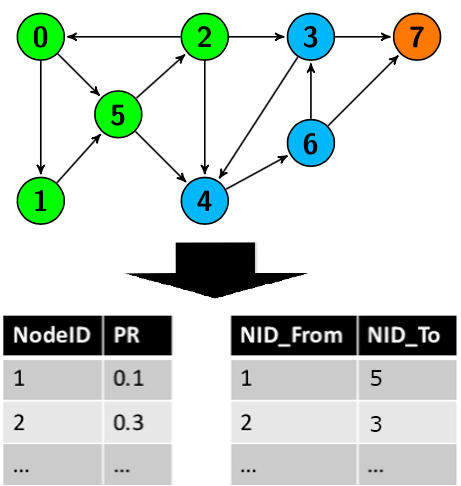
\includegraphics[width=0.4\textwidth]{./ImagenesMemoria/TablaEjemplo}
    \caption{\label{fig:tablaEj}Ejemplo de Grafo}
\end{figure}


Para la realización de este trabajo se ha hecho uso del entorno de desarrollo Jupyter y de la herramienta notebook. El código está escrito mediante el lenguaje de programación Python, usando principalmente las librerías pandas, NetworkX y scikit-learn, y otras como keras, tensorflow y matplot.



Los modelos de clasificación usados son: KNN, Naive Bayes, Árboles de Decisión y Redes Neuronales.

\section{Conjunto de datos y Tarea de predicción a realizar}
Hemos elegido un dataset (fíjese en la Fig. \ref{fig:dataset}) de la página de streamings en directo twitch.tv, en la que se ve: las visitas, días (ambos de tipo entero) que transmitido un canal en directo, si tiene contrato o no con twitch (partner de tipo Boolean) y si el contenido del canal (id de tipo Integer) es o no para adultos (mature de tipo Boolean). Al ser la propia Twitch la que ofrece este contrato, hemos decidido que la predicción para nuestros modelos sea el atributo partner (true/false). Las aristas (edges) representan si dos usuarios tienen una relación de amistad.

\begin{figure} % opción de posicionamiento
    \centering
    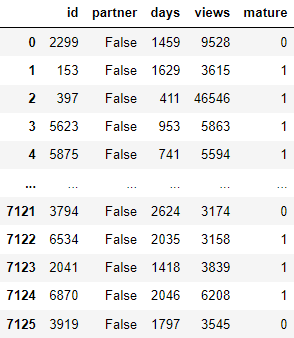
\includegraphics[width=0.3\textwidth]{./ImagenesMemoria/dataset}
    \caption{\label{fig:dataset}Tabla de Datos}
\end{figure}

Este dataset tenía dos tipos de id asociados a cada usuario, uno generado aleatoriamente y otro donde al usuario se le asignaba un valor entre 0 y el numero total de usuarios que recoge el conjunto de datos, por lo que decidimos que eliminar el id generado de forma aleatoria para mayor claridad y sólo hace falta un id por usuario para identificarlos.


Para este estudio hemos decidido que el atributo a predecir será partner. Para ello, haremos uso de los atributos: days, views y mature (el id no es relevante en este caso). Lo hemos planteado como una tarea de clasificación binaria, ya que partner solo tiene dos valores posibles (True o False).

 Por último hemos codificado (codificación one-hot) los valores de mature de Booleano a Integer, pasando True-False a 1-0 respectivamente, para que sea más eficiente estimar las probabilidades del atributo partner.

\section{Métricas Relacionales}
Como este es un trabajo de desarrollo de modelos orientados al aprendizaje automático grafos, hemos elegido una serie de métricas relacionales que aplicaremos como atributos relacionales. En concreto hemos elgido tres métricas:

\begin{enumerate}
\item\textbf{Betweenness centrality} (Centralidad de intermediación): La centralidad en un grafo puede ser entendida como una medida que determina la relevancia de un nodo dentro del grafo y permite comparar o contrastar dicho vértice con otros. La Betweenness Centrality es una medida de centralidad que cuantifica la frecuencia en la que un nodo se encuentra en el camino más corto entre dos nodos determinados. Cuando en un grafo existen nodos de alta intermediación, estos suelen jugar un rol importante en la estructura a la que pertenecen. Estos nodos también poseen capacidades de ser controladores o reguladores de los flujos de información dentro de la estructura total del grafo. 
\item\textbf{Clustering} (agrupamiento): es una tarea que tiene como finalidad principal lograr el agrupamiento de nodos, para lograr construir subconjuntos de datos conocidos como Clusters.
\item\textbf{Degree} (grado): Número de aristas (relaciones) que inciden sobre el nodo.
\end{enumerate}
 
\section{Algoritmos de Aprendizaje Automático}
A continuación exponemos los algoritmos que hemos utilizado con nuestro dataset:

\subsection{KNN}
El algoritmo kNN (del inglés \emph{k Nearest Neighbors}, k vecinos más cercanos), es un clasificador de aprendizaje supervisado no paramétrico, por lo que la cantidad de parámetros del modelo coincide exactamente con la cantidad de ejemplos de entrenamiento. Se basa en la proximidad de los k nodos más cercanos calculando la cercanía a partir de los atributos, si estos fueran discretos sería necesaria una codificación de los mismo. 

Analizando nuestro dataset, se puede observar como el atributo "\emph{views}" toma valores de mayor magnitud con respecto al resto lo que provoca que tenga más en cuenta para la predicción del modelo. Con el fin de evitar esta situación se hace uso de la normalización a los atributos del conjunto de entrenamiento. Existe una gran variedad de maneras de normalizar un atributo numérico, nosotros hemos optado por el método min-max \cite{b1} que consiste en que a cada atributo restarle el valor mínimo de este y dividir esta diferencia entre la resta del valor máximo y mínimo: 

\begin{equation}
v_{i}' = \frac{v_{i} - m}{M - m}
\end{equation}

Para realizar kNN es necesario dar un valor al hiperparámetro k, referido al número de vecinos que se va a tener en cuenta a la hora de clasificar un nuevo dato, nosotros le hemos dado valores del uno al diez para más tarde evaluar el rendimiento de cada uno y elegir el mejor. También existen métodos para calcular la distancia, en nuestro caso hemos usado:
\begin{itemize}
\item Distancia de \emph{Hamming} para el dataset sin atributos relacionales:
\begin{equation}
d(\textbf{x},\textbf{x}') = \sum_{i=1}^n \mathbbm{1}{(x_{i}\neq{x_{i}'})}
\end{equation}
Hemos usado esta métrica ya que según la docmentación de la librería \cite{b2} es la recomendada para valores enteros.
\\
\item Distancia \emph{Manhattan} para el dataset con atributos relacionales:
\begin{equation}
d(\textbf{x},\textbf{x}') = \sum_{i=1}^n |x_{i} - x_{i}'|
\end{equation}
En este caso es la adecuada al tratarse de valores numéricos reales.
\end{itemize}

Para el cálculo del modelo ha sido necesaria la clase neighbors de la librería sklearn.
Por último, una vez se ha construido el modelo lo evaluamos mediante validación cruzada (cross validation) con 10 pliegues. Se divide el dataset según el numero de pliegues, siendo uno de estos el que se usará para probar el modelo y el resto para entrenarlo, de tal manera que cada pliegue acabe siendo usado como subconjunto de prueba. Cada una de estas iteraciones dará como resultado una tasa de acierto, la media de estas será el valor asociado a cada k. Finalmente se comparan y se escoge el valor de k que obtuviera la media la más alta.

\subsection{Naive Bayes}
Naive Bayes se trata de un modelo de clasificación paramétrico, ya que no depende de la cantidad de ejemplos que contega el conjunto de entrenamiento. Los valores deben ser discretos, y en caso contrario deberán someterse a un proceso de discretización, donde se divide el rango de los valores de los atributos en subintervalos, los cuales constituiran los posibles valores de la variable discretizada. En nuestro era necesaria la discretización al tratarse de enteros con una gran diferencia entre los valores.
Para realizar la tarea de clasificación se aprende primero los siguientes valores de los parámetros:
\begin{itemize}
\item La probabilidad de cada clase c:
\begin{equation}
\mathbbm{P}(c) = \frac{ N_{c}}{N}
\end{equation}
Donde $N_{c}$ es la cantidad total de ejemplos que pertenecen a la clase c, y N la cantidad total de los ejemplos que hay en el conjunto de entrenamiento.
\\ 
\item La probabilidad de para cada atributo X, cada posible valor de x el atributo y cada clase c:
\begin{equation}
\mathbbm{P}(X = x | c) = \frac{N_{X=x,c}}{N{c}}
\end{equation}
Donde $N_{X=x,c}$  es la cantidad total de ejemplos del conjunto de entrenamiento que pertenecen a la clase c en los que el atributo X toma el valor x.
\end{itemize}

A la hora de discretizar los atributos hemos usado KBinsDiscretizer \cite{b3}, de la libretria sklearn. Para los parámetros usamos una codificación one-hot, ya que algunos atributos tiene valores numéricos muy elevados comparados con otros. Por esta razón hemos elgido esta codificación, pues proporciona mejor resultado que otras (como por ejemplo la de tipo ordinal).

A la hora de construir el modelo se ha usado MultinomialNB(alpha=k)  \cite{b4}, pues es el más apropiado para clasificación de atributos numéricos discretizados. El hiperparámetro usado, k, se usa para realizar el suavizado de Laplace. Dicho suavizado se realiza cuando alguna de las probabilidades calculadas para una clase c toma el valor 0, haciendo que un ejemplo nunca se clasifique en dicha clase c. La fórmula que nos indica el suavizado de Laplace es la siguiente:
\begin{equation}
\mathbbm{P}(X = x | c) = \frac{N_{X=x,c}+1}{N_{c} + k|X|}
\end{equation}

Para la evaluación de este modelo también hemos usado el método de validación cruzada con 10 pliegues.

\subsection{Árboles de Decisión}

Los Árboles de Clasificación y regresión (del inglés CART, clasification and regresion tree) son modelos para adecuados para tareas de tanto de clasificación como de regresión dados atributos necesariamente numéricos, ya sean continuos o discretos.En un CART cada nodo interno está etiquetado con un atributo y un valor umbral para dicho atributo, mientras que cada hoja está etiquetada con una clase si es una tarea de clasificación, o un número en caso de que se trate de una tarea de regresión.  Dado nuestro conjunto de datos, la tarea a abordar es una de clasificación, por lo que elegimos el tipo de árbol correspondiente.

El algoritmo CART para el aprendizaje del modelo es tal que dado un conjunto de ejemplos de entrenamiento $\mathscr{D}$, denotamos  $\mathscr{D}_n$ al subconjunto de ejemplos que satisfacen  todas las condiciones de los nodos desde la raíz hasta hasta n. Dado un nodo $n$ un atributo $X$, siendo $x_1$, $x_2$, ... , $x_k$  la secuencia de distintos valores que toma $X$ en $\mathscr{D}_n$, estando estos ordenados de menor a mayor. Siendo $u_i = \frac{(x_i + x_{i+1})}{2} $ el umbral candidato para $X$ y con $i$ en el rango $(1, 2, ..., k-1)$. A continuación se divide  $\mathscr{D}_n$ según el umbral. Si los ejemplos de $X$ toman un valor menor o igual que $u$ estos se agrupan en  $\mathscr{D}_n^{Izq}$, mientras que si son mayores que $u$ se agruparan en en el subconjunto $\mathscr{D}_n^{Der}$. Por último, se hace uso de una función $I$ que permite medir la impureza de un conjunto de ejemplos, para poder elegir el par $(X, u)$ que nos de una mejor partición de  $\mathscr{D}_n$, siendo dicha función:

\begin{equation}
\textbf{arg mín  } \frac{|\mathscr{D}_{n}^{Izq}|}{|\mathscr{D}|}I(\mathscr{D}_{n}^{Izq})+ \frac{|\mathscr{D}_{n}^{Der}|}{|\mathscr{D}|}I(\mathscr{D}_{n}^{Der})
\end{equation}

Una representación del algoritmo sería:

\begin{pseudo}*
    \hd{CART}(\mathscr{D}) \\
    \textbf{Si} \textnormal{\fn{NODIVISIBLE($\mathscr{D}$)}} \textbf{entonces} \\+
    \textbf{Devolver} \textnormal{un nodo etiquetado con \fn{ETIQUETA}(\mathscr{D})} \\-
    Si no entonces \\+
    \(\textnormal{Elegir el par $(X, u)$ que proporcione la mejor partición $(\mathscr{D}^{Izq},\mathscr{D}^{Der})$ de $\mathscr{D}$}\) \\
    \( T_{1} \leftarrow \textnormal{CART($\mathscr{D}^{Izq}$)}\) \\
    \( T_{2} \leftarrow \textnormal{CART($\mathscr{D}^{Der}$)}\) \\
    \(\textbf{Devolver } \textnormal{un nodo etiquetado con ($X, u$) y cuyos hijos sean $T_{1}$  y $T_{2}$}\)\\
 \end{pseudo}



\begin{figure} % opción de posicionamiento
    \centering
    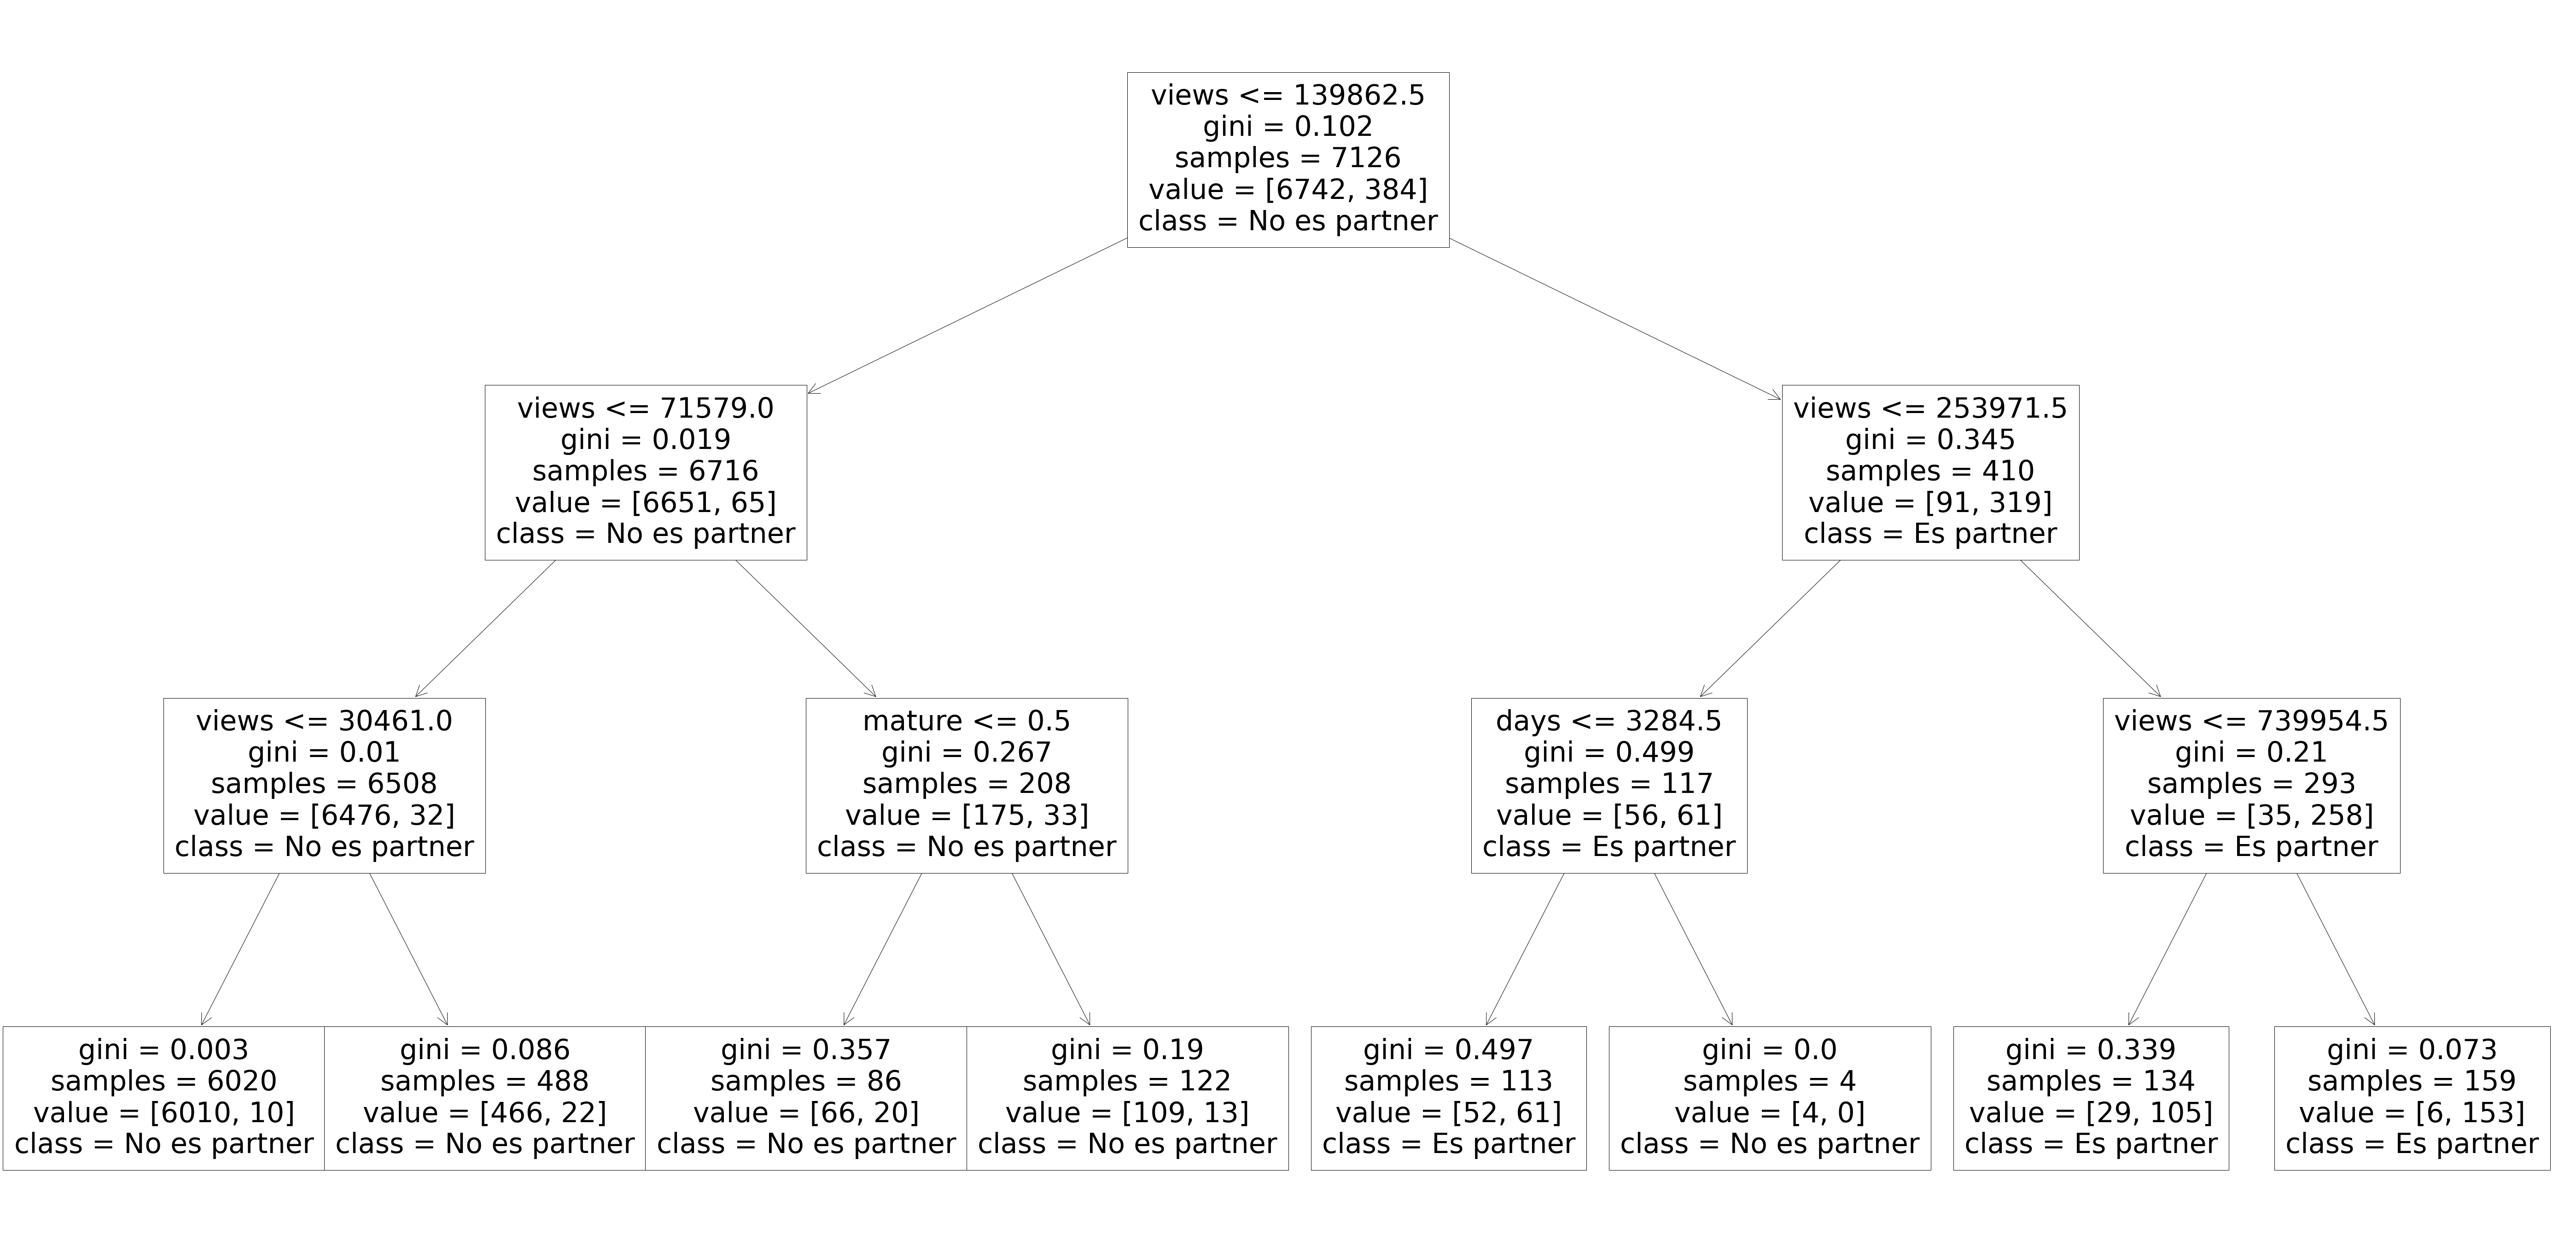
\includegraphics[width=0.5\textwidth]{./ImagenesMemoria/Arbol}
    \caption{\label{fig:arbolDecision}Árbol de Decisión}
\end{figure}

 La función de impureza usada para una tarea de clasificación suele serel índice de Gini, pues estima la probabilidad de clasificar incorrectamente un ejemplo. Tal que: 
\begin{equation}
G(\mathscr{D}) = \sum_{c\in C} \hat{\pi}_c (1-  \hat{\pi}_c) = 1 -  \sum_{c\in C}  \hat{\pi}_c^2
\end{equation}

Para abordar esta tarea hemos hecho uso de las librerías sklearn y matplotlib para mostrar el árbol resultado por pantalla. Dada la naturaleza hemos decidido usar la función DecisionTreeClassifier de la clase tree, puesto que nos proporciona un árbol de decisión el cual ha sido limitado a una profundidad máxima de 5. Para terminar, realizamos una evaluación del modelo mediante el método score, que calcula el rendimiento del modelo, dados por separado el conjunto de ejemplos de prueba y la clase de cada uno de estos ejemplos.


\subsection{Redes Neuronales}


\section{Resultados}

En esta sección se detallarán tanto los experimentos realizados como los
resultados conseguidos:
\begin{itemize}
\item Los experimentos realizados, indicando razonadamente la configuración
  empleada, qué se quiere determinar, y como se ha medido.
\item Los resultados obtenidos en cada experimento, explicando en cada caso lo
  que se ha conseguido.
\item Análisis de los resultados, haciendo comparativas y obteniendo
  conclusiones.
\end{itemize}

Se pueden hacer uso de tablas, como el ejemplo de la tabla~\ref{tab:ejemplo}.




\section{Conclusiones}

Finalmente, se dedica la última sección para indicar las conclusiones obtenidas
del trabajo. Se puede dedicar un párrafo para realizar un resumen sucinto del
trabajo, con los experimentos y resultados. Seguidamente, uno o dos párrafos
con conclusiones. Se suele dedicar un párrafo final con ideas de mejora y
trabajo futuro.


\section{Bibliografía}
\begin{thebibliography}{00}
\bibitem{b1} \url{https://scikit-learn.org/stable/modules/preprocessing.html#normalization}
\bibitem{b2} \url{https://scikit-learn.org/stable/modules/generated/sklearn.metrics.DistanceMetric.html}
\bibitem{b3} \url{https://scikit-learn.org/stable/modules/generated/sklearn.preprocessing.KBinsDiscretizer.html}
\bibitem{b4} \url{https://scikit-learn.org/stable/modules/generated/sklearn.naive_bayes.MultinomialNB.html}
\bibitem{b5} \url{https://scikit-learn.org/stable/modules/naive_bayes.html}
\end{thebibliography}


\end{document}
